%!TEX program = xelatex
%!TEX TS-program = xelatex
%!TEX encoding = UTF-8 Unicode

\documentclass[a4paper, 12pt, centering]{article}



% ===========================页面设置===============================================
\usepackage{geometry}   %设置页边距的宏包
\geometry{left=2.5cm,right=2cm,top=2.5cm,bottom=2.5cm}  %设置 上、左、下、右 页边距

\usepackage{graphicx}  %插入图片的宏包
\usepackage{float} %设置图片浮动位置的宏包
\usepackage{subfigure} %插入多图时用子图显示的宏包
\usepackage[unicode]{hyperref} %超链接,支持unicode字符
\hypersetup{hidelinks} %隐藏超链接上的外框
\usepackage{xcolor}
\usepackage{indentfirst} %自动缩进

\usepackage{wallpaper} %background image
\addtolength{\wpYoffset}{8.0cm}
\usepackage{url}
\usepackage{fontspec,xltxtra,xunicode}
\defaultfontfeatures{Mapping=tex-text} %如果没有它,会有一些 tex 特殊字符无法正常使用,比如连字符
%文章内中文自动换行,可以自行调节
\XeTeXlinebreaklocale “zh”
\XeTeXlinebreakskip = 0pt plus 1pt minus 0.1pt

%%%% 下面的命令设置行间距与段落间距 %%%%
\linespread{1.4}
% \setlength{\parskip}{1ex}
\setlength{\parskip}{0.5\baselineskip}




% ===========================中文字体支持===============================================
% 字体需要根据自己电脑系统来设置
\usepackage{xeCJK}
\setmainfont{Times New Roman}
\setCJKmainfont{宋体}

\setCJKfamilyfont{zhhei}{黑体}
\newcommand*{\hei}{\CJKfamily{zhhei}}
\setCJKfamilyfont{zhkai}{楷体}
\newcommand*{\kai}{\CJKfamily{zhkai}}
\setCJKfamilyfont{enroman}{Times New Roman}
\newcommand*{\mytimes}{\CJKfamily{enroman}}




% ===========================数学符号===============================================
\usepackage{amsmath,amssymb}
\usepackage{bm} % $\bm{letter}$ 数学式中粗斜体字母的最佳方案
\usepackage{calc}
\usepackage{units} %单位宏包



% ===========================字号===============================================
\newcommand{\chuhao}{\fontsize{42pt}{\baselineskip}\selectfont}
\newcommand{\xiaochuhao}{\fontsize{36pt}{\baselineskip}\selectfont}
\newcommand{\yihao}{\fontsize{28pt}{\baselineskip}\selectfont}
\newcommand{\erhao}{\fontsize{21pt}{\baselineskip}\selectfont}
\newcommand{\xiaoerhao}{\fontsize{18pt}{\baselineskip}\selectfont}
\newcommand{\sanhao}{\fontsize{15.75pt}{\baselineskip}\selectfont}
\newcommand{\sihao}{\fontsize{14pt}{\baselineskip}\selectfont}
\newcommand{\xiaosihao}{\fontsize{12pt}{\baselineskip}\selectfont}
\newcommand{\wuhao}{\fontsize{10.5pt}{\baselineskip}\selectfont}
\newcommand{\xiaowuhao}{\fontsize{9pt}{\baselineskip}\selectfont}
\newcommand{\liuhao}{\fontsize{7.875pt}{\baselineskip}\selectfont}
\newcommand{\qihao}{\fontsize{5.25pt}{\baselineskip}\selectfont}



% ===========================定义摘要、关键词、章节等命令===============================================
\makeatletter
\renewcommand\abstract{%
\kai\textbf{\hei{摘要:}}
{\normalfont\xiaosihao\kai}}
\makeatother

\newenvironment{enabstract}

\makeatletter
\renewcommand\enabstract{%
\textbf{Abstract: }
{\normalfont\xiaosihao\mytimes}}
\makeatother

%%%% 设置 key words 属性 %%%%
\newenvironment{keys}

\makeatletter
\renewcommand\keys{%
\kai\textbf{\hei{关键词:}}
{\normalfont\xiaosihao\hei}}
\makeatother

\newenvironment{enkeys}

\makeatletter
\renewcommand\enkeys{%
\textbf{Key words: }
{\normalfont\xiaosihao\mytimes}}
\makeatother

%%%% 设置 section 属性 %%%%
\makeatletter
\renewcommand\section{\@startsection{section}{1}{\z@}%
{-1.5ex \@plus -.5ex \@minus -.2ex}%
{.5ex \@plus .1ex}%
{\normalfont\sihao\bf\hei}}
\makeatother

%%%% 设置 subsection 属性 %%%%
\makeatletter
\renewcommand\subsection{\@startsection{subsection}{1}{\z@}%
{-1.25ex \@plus -.5ex \@minus -.2ex}%
{.4ex \@plus .1ex}%
{\normalfont\xiaosihao\bf\hei}}
\makeatother

%%%% 设置 subsubsection 属性 %%%%
\makeatletter
\renewcommand\subsubsection{\@startsection{subsubsection}{1}{\z@}%
{-1ex \@plus -.5ex \@minus -.2ex}%
{.3ex \@plus .1ex}%
{\normalfont\xiaosihao\hei}}
\makeatother

%%%% 段落首行缩进两个字 %%%%
\makeatletter
\let\@afterindentfalse\@afterindenttrue
\@afterindenttrue
\makeatother
\setlength{\parindent}{2em}  %中文缩进两个汉字位






%%%% 定理类环境的定义 %%%%
\newtheorem{example}{例}             % 整体编号
\newtheorem{algorithm}{算法}
\newtheorem{theorem}{定理}[section]  % 按 section 编号
\newtheorem{definition}{定义}
\newtheorem{axiom}{公理}
\newtheorem{property}{性质}
\newtheorem{proposition}{命题}
\newtheorem{lemma}{引理}
\newtheorem{corollary}{推论}
\newtheorem{remark}{注解}
\newtheorem{condition}{条件}
\newtheorem{conclusion}{结论}
\newtheorem{assumption}{假设}

%%%% 重定义 %%%%
\renewcommand{\contentsname}{目录}  % 将Contents改为目录
\renewcommand{\abstractname}{摘要}  % 将Abstract改为摘要
\renewcommand{\refname}{参考文献}   % 将References改为参考文献
\renewcommand{\indexname}{索引}
\renewcommand{\figurename}{图}
\renewcommand{\tablename}{表}
\renewcommand{\appendixname}{附录}
\renewcommand{\algorithm}{算法}


%%%% 定义标题格式,包括title,author,affiliation,email等 %%%%
\title{\yihao{模式识别报告}}
\author{\sanhao XiaoX\\[2ex]
\sanhao Demon Killer\\[2ex]
}
\date{\sanhao\today}




% ===========================正正正正正正正==============================================
% ===========================文文文文文文文===============================================
% ===========================这这这这这这这===============================================
% ===========================里里里里里里里===============================================
% ===========================开开开开开开开===============================================
% ===========================始始始始始始始===============================================
% ===========================写写写写写写写===============================================
% ===========================哟哟哟哟哟哟哟===============================================



\begin{document}

%封面背景图片
%可以换其它自己想放的图片
\ThisCenterWallPaper{0.5}{tju.png}



%%%% 以下部分是正文 %%%%

%标题上方空出一些距离
\
\vspace{10cm}
\begingroup
\let\newpage\relax% Void the actions of \newpage
\maketitle
\endgroup
\newpage
%----------


%%% 摘要 %%%

\begin{abstract}
论文选自CVPR2022的一篇,题目为《HCSC: Hierarchical Contrastive Selective Coding》。来自上海交通大学、Mila 魁北克人工智能研究所以及字节跳动的研究者提出了一种具有层级语义结构的自监督表征学习框架,在 ImageNet 数据集上预训练的模型在多个下游任务中取得了 SOTA 性能。\\
本报告将从文章概要,研究背景,知识联系,个人收获几方面做简要汇报。
\end{abstract}

\begin{keys}
关键词1;关键词2;关键词3
\end{keys}

% \begin{enabstract}
% Here is English abstract. Here is English abstract. Here is English abstract. Here is English abstract. Here is English abstract. Here is English abstract. Here is English abstract. Here is English abstract. Here is English abstract. Here is English abstract. Here is English abstract. Here is English abstract. Here is English abstract. Here is English abstract. Here is English abstract. Here is English abstract. Here is English abstract. Here is English abstract. Here is English abstract. Here is English abstract.
% \end{enabstract}

% \begin{enkeys}
% keyword1, keyword2, keyword3
% \end{enkeys}
\newpage

%%% 目录 %%%
\tableofcontents
\newpage

\section{文章概要}
自然界中广泛存在如图1这种分层的语义概念,比如哺乳动物--狗--拉布拉多,相似图片可能在某个层次上属于同一分类。这种现象在image的数据集上是广泛存在的,如果能引入这样的信息会有助于预训练模型迁移到下游任务上。
\begin{figure}[H] %H为当前位置,!htb为忽略美学标准,htbp为浮动图形
\centering %图片居中
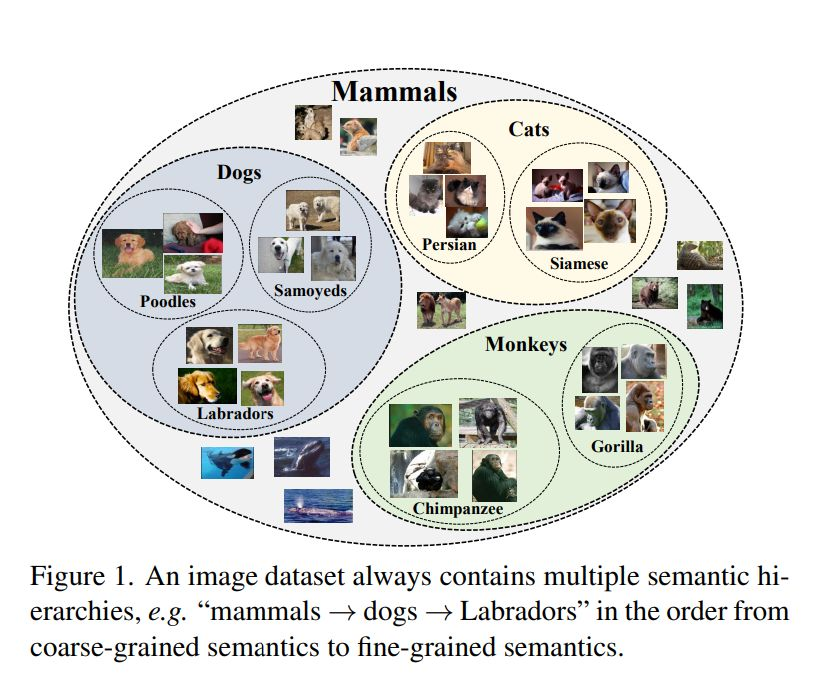
\includegraphics[width=0.8\textwidth]{Fig1.jpg} %插入图片,[]中设置图片大小,{}中是图片文件名
\label{Fig.main} %用于文内引用的标签
\end{figure}
现有的对比学习模型,作者认为存在以下的问题:\\
1.缺乏对上述描述的分层语义结构的建模\\
2.对比学习中的负样本不能保证语义是不同的,妨碍了模型的学习\\

因此本文作者提出了Hierarchical Contrastive Selective Coding (HCSC)模型,模型为了解决现有存在的问题,建立了一组动态更新的层次原型,以表示潜在空间中数据的层次语义结构,在训练过程中可以选择更合适的对比样例进行训练。
\subsection{研究背景}
\subsubsection{MoCo}
对比学习($\color{red}{Co}\color{black}{ntrastive\ Learning}$),顾名思义就是对比着进行学习。不需要知道标签的具体信息,因此这是一种无监督学习方法。目的是将类似的图片的特征在特征空间中尽量的靠近,即缩小与正样本间的距离,扩大与负样本间的距离。
Moco将一系列的对比学习方法归纳为一个字典查询的问题。从动态字典的角度看对比学习,相当于在字典中查询,相似的query和key应尽量靠近。要想获得较好的训练结果,字典应该满足大且保持一致性两个特征。
\begin{figure}[H] %H为当前位置,!htb为忽略美学标准,htbp为浮动图形
\centering %图片居中
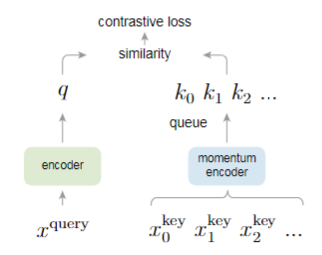
\includegraphics[width=0.8\textwidth]{Moco_Figure_1.png} %插入图片,[]中设置图片大小,{}中是图片文件名
\label{Fig.1} %用于文内引用的标签
\end{figure}
Moco在不断更新encoder的过程中提出了两点优化策略:
1.使用队列结构存储字典中的键值(负样本),由于训练中每个batch在不断$push\_back$和$pop\_front$,总体来看这个字典就能变得非常大。
2.引入动量($\color{red}{Mo}\color{black}{mentum}$)参数保证momentum encoder的缓慢变化,从而保证key的一致性。
$$
    \theta_k=m\theta_{k-1}+(1-m)\theta_q
$$

\subsubsection{PCL}
PCL是对MoCo的改进,他认为MoCo只把自己当作正样本,其他样本均当作负样本的操作太过暴力,毕竟其他样本中有很多都是相似样本。
所以作者提出先将样本聚类,自己的聚类中心(也就是所谓原型)当作正原型,其他原型当作负原型,拉近正原型,推开负原型。
聚类采用k-means,作者采用了不同的k值求loss取平均。
框架是EM框架,
E步:根据上一轮动量编码的输出结果计算距离进行k-means聚类,计算出原型c和浓度ϕ。
M步:将计算出的原型c和浓度ϕ带入到下一轮loss计算中并进行更新。

这种方法站在聚类后的类层次上的,获得聚集在相应的集群中心周围的紧凑的图像表示,从而捕获一些可以由单一集群层次表示的基本语义结构。
PCL不仅学习低级特征来完成实例识别任务,更重要的是将聚类发现的语义结构编码到学习的嵌入空间中。

\subsubsection{HCSC}
HCSC是在PCL上的进一步改进工作。他认为PCL直接将多粒度原型对比学习的loss取平均太过暴力。不同粒度间是有关联的,就比如自然界,哺乳动物--狗--拉布拉多,就是一个粒度的关联。所以作者进行如下改进,对于PCL采用不同k值的k-means的并行操作,作者改成了串行操作,即对聚类产生的原型,将原型进行再次聚类,(框架仍然是EM框架),这样循环聚类L次产生树结构。在采样负样本的时候,根据树结构计算每层的样本距离,根据距离来采样负样本和负原型,加入计算中。
\subsection{知识联系}
总体来说这一系列研究都与Feature Selection和Feature Extraction有关,是为后期应用于分类,检测,分割等下游任务的pre-train工作,来提取出更加有效的特征。
\section{文章内容}
\subsection{实验方法}
该工作的方法论框架包含两个重要的模块: 一个是层级语义结构的构建与维护, 另一个是基于层级语义结构的选择性对比学习。
\subsubsection{层级语义表征}
层级语义结构天然可以通过树状结构来描述:如果将树中的某个节点认为是一个语义类别, 则父节点可以认为是它的上层类别。如下图(a)中,「拉布拉多犬」的父节点是「犬类」,而其兄弟节点可以包括「贵宾犬」等。这样的树状结构显然具备一个性质:同一父节点的两个子节点必然也共享更上层的祖先节点,例如「贵宾犬」与「拉布拉多犬」同为犬类, 它们也同为哺乳动物。
\begin{figure}[H] %H为当前位置,!htb为忽略美学标准,htbp为浮动图形
    % \centering %图片居中
    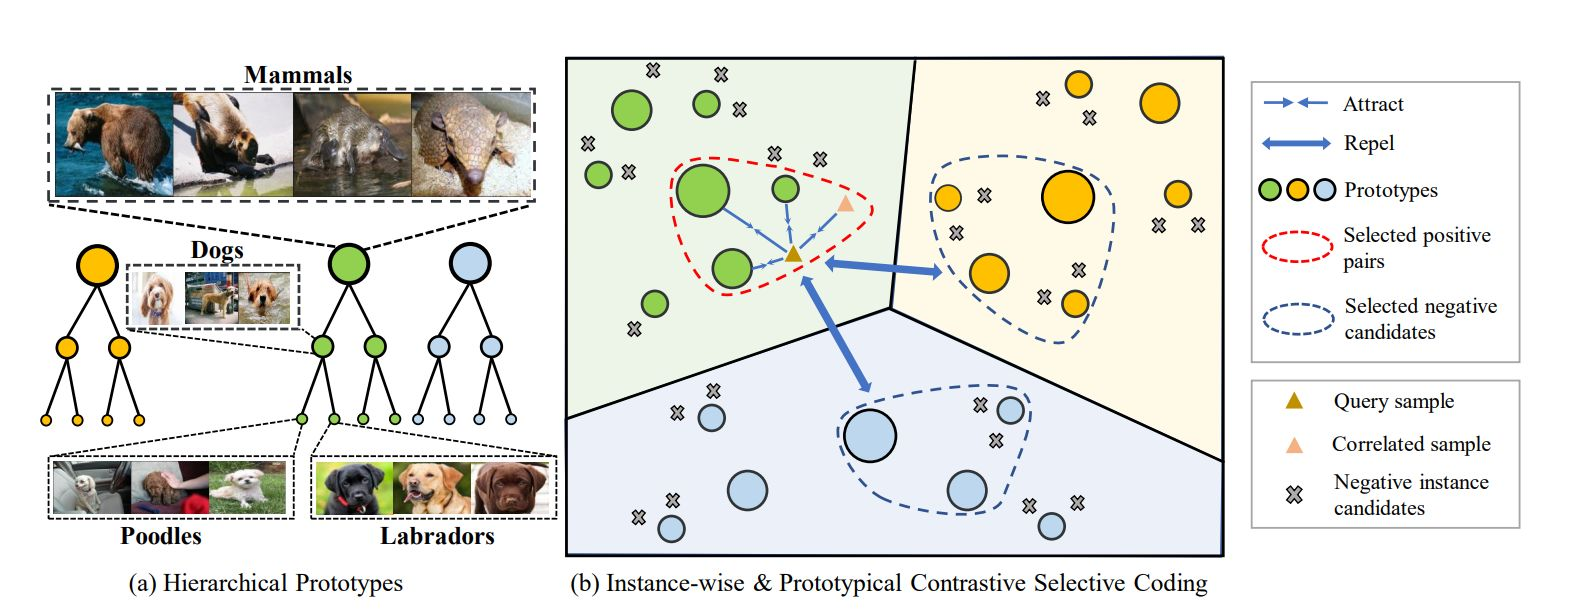
\includegraphics[width=1.1\textwidth]{Fig3.jpg} %插入图片,[]中设置图片大小,{}中是图片文件名
    \label{Fig.3} %用于文内引用的标签
\end{figure}
可以通过对图像特征聚类的方式获得图像的潜在语义类别。聚类中心则可以被认为是代表着某种语义类别的“原型”,基于自底向上的层级聚类思想, 在这些聚类中心的基础上进一步进行聚类则可以得到更高层级的潜在语义类别。在这一过程中, 语义类别的树状结构自然地得以维护。

下图为论文中采用的层次K-means聚类算法的流程图,对聚类产生的原型,将原型进行再次聚类,一共L次,最终形成一棵树的结构。
\begin{figure}[H] %H为当前位置,!htb为忽略美学标准,htbp为浮动图形
    \centering %图片居中
    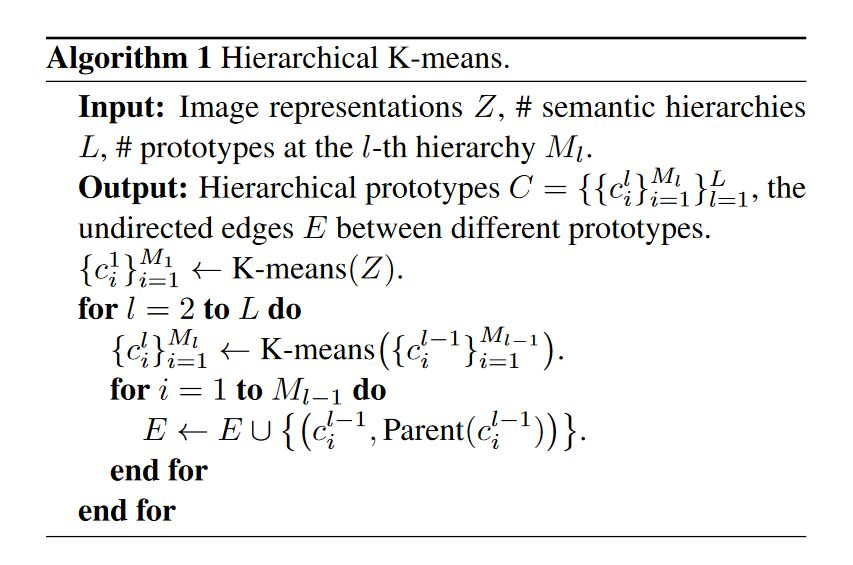
\includegraphics[width=0.8\textwidth]{Fig2.jpg} %插入图片,[]中设置图片大小,{}中是图片文件名
    \label{Fig.2} %用于文内引用的标签
\end{figure}
\subsubsection{选择性对比学习}
有了层级信息,则可以在实例(Instance-wise)对比学习中指导负样本的选取,通过每次聚类形成的标签,将同类型(属于相同聚类中心)的负样本剔除。
下图为训练过程中,对于不同的query,删除的同类型负样本
\begin{figure}[H] %H为当前位置,!htb为忽略美学标准,htbp为浮动图形
    \centering %图片居中
    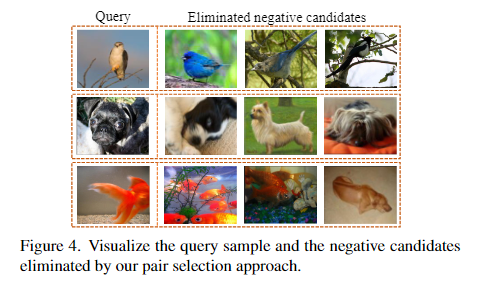
\includegraphics[width=\textwidth]{Fig4.png} %插入图片,[]中设置图片大小,{}中是图片文件名
    \label{Fig.4} %用于文内引用的标签
\end{figure}
类似地,层级原型还可用于辅助原型(Prototypical)对比学习,原型对比学习是图像表征与聚类中心之间的交互,在选取负原型时,可以尽量避免选取与当前聚类中心语义相近的原型,表现在树形结构上就是尽量避免选取当前节点的兄弟节点。
具体来说,可以计算候选原型$c_j$与目标原型$c^l(z)$父节点的相似程度,相似度大的则减小其选中的概率。
$$
    p^l_{Select}(c_j;c^l(z))=1-\frac{\exp [s(c_j,Parent(c^l(z)))]}{\sum_{i=1}^{M_{l+1}}\exp [s(c_j,c^{l+1}_i)]}
$$
将两种改进后的对比学习损失进行组合得到最终的优化目标
$$
    \mathcal{L}=\mathcal{L}_{ICSC}+\mathcal{L}_{PCSC}
$$

\subsection{实验结论}
对各种下游任务的大量实验验证了HCSC方法的优越性。该论文还给出了直观的可视化结果。在论文中结论部分展示了 HCSC 在 ImageNet 上的聚类结果,在下图中可以明显地看出存在层级结构:叼着鱼的灰熊 => 在水上的熊或者狗 => 在水上的动物。
\begin{figure}[H] %H为当前位置,!htb为忽略美学标准,htbp为浮动图形
    \centering %图片居中
    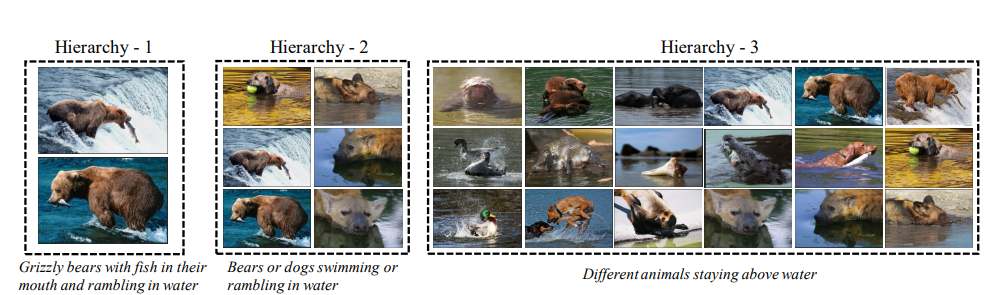
\includegraphics[width=\textwidth]{Fig5.png} %插入图片,[]中设置图片大小,{}中是图片文件名
    \label{Fig.5} %用于文内引用的标签
\end{figure}
\section{个人体会}
模式识别作为人工智能的一个分支领域,上世纪50年代以来逐渐形成了
理论方法体系并快速发展,提出了统计模式识别、句法结构模式识别、神经网络、
深度学习等多种有效的理论与方法,应用上也取得了巨大进展,尤其是视
觉模式识别。然而,面向复杂开放环境、小样本、动态场景等挑战,当前依赖大数
据学习的主流方法在泛化性、自适应性等方面存在明显不足。这篇论文在自监督学习方面
做出了一定贡献,从分类学中不同层级的角度出发,将原型之间以树形结构联系起来,同时结合前人的研究成果,将PCL和MoCo的针对样本和原型的对比学习方法结合起来,取得了较好的成果,开阔了我的思维和眼界。

\begin{thebibliography}{1}
    \bibitem{1} Kaiming He et al. “Momentum Contrast for Unsupervised Visual Representation Learning” arXiv: Computer Vision and Pattern Recognition (2019): n. pag.
    \bibitem{2} Junnan Li et al. “Prototypical Contrastive Learning of Unsupervised Representations” Learning (2020): n. pag.
    \bibitem{3} Y. Guo et al., "HCSC: Hierarchical Contrastive Selective Coding," 2022 IEEE/CVF Conference on Computer Vision and Pattern Recognition (CVPR), 2022, pp. 9696-9705, doi: 10.1109/CVPR52688.2022.00948.
\end{thebibliography}

\end{document}
